% ***************************************************************************************************
%
%	Szablon pracy magisterskiej dla Politechniki Wrocławskiej w wersji dwustronnej.
%	Autor:	Tomasz Strzałka
%
% ***************************************************************************************************

% Styl dwustronny z domyślną wielkością czcionki 10pt oraz oddzieloną stroną tytułową (titlepage).
% Domyślnie rodziały rozpoczynają się na stronie prawej (openright).
\documentclass{book}

% ***************************************************************************************************
% Ustawienia języka
% ***************************************************************************************************

% Podstawowe ustawienia języka, według którego formatowany będzie dokument
\usepackage[polish]{babel}

% Pakiet babel dla polskiego języka powoduje konflikt z pakietem amssymb.
% Polecenie '\lll' definiują oba pakiety - porządana jest druga definicja.
\let\lll\undefined

% W przypadku wielojęzykowości ustawia główny język dokumentu
\selectlanguage{polish}

% Kodowanie dokumentu
\usepackage[utf8]{inputenc}

% Dowolny rozmiar czcionek, kodowanie znaków
\usepackage{lmodern}

% Polskie wcięcia akapitów
\usepackage{indentfirst}

% Polskie łamanie wyrazów
\usepackage[plmath]{polski}

% Przecinek w wyrażeniach matematycznych zamiast kropki
\usepackage{icomma}

% Polskie formatowanie typograficzne
\frenchspacing

% Zapewnia liczne usprawnienia wyświetlania i organizacji matematycznych formuł. 
\usepackage{amsmath}

% Wprowadza rozszerzony zestaw symboli m.in. \leadsto
\usepackage{amssymb}

% Dodatkowa, ,,kręcona'' czcionka matematyczna
\usepackage{mathrsfs}

% Dodatkowe wsparcie dla środowiska mathbb, które nie wspiera domyślnie cyfr (\mathbb{})
\usepackage{bbold}

% Fixes/improves amsmath
\usepackage{mathtools}


% ***************************************************************************************************
% Kolory  
% ***************************************************************************************************

% Umożliwia kolorowanie poszczególnych komórek tabeli
\usepackage[table]{xcolor}% http://ctan.org/pkg/

% Umożliwia łatwą zmianę koloru linii w tabeli
\usepackage{tabu}

% Umożliwia rozszerzoną kontrolę nad kolorami.
\usepackage{xcolor}

% Definicje kolorów
\definecolor{lgray}{HTML}{9F9F9F}
\definecolor{dgray}{HTML}{5F5F5F}
% lgray				-	nazwa nowo zdefiniowanego koloru
% HTML				-	model kolorów
% CCCCCC			-	wartość koloru zgodna z modelem

% ***************************************************************************************************
% Algorytmy 
% ***************************************************************************************************

% Udostępnia środowisko do konstruowania pseudokodów
\usepackage[ruled,vlined,linesnumbered,longend,algochapter]{algorithm2e}
% ruled	- poziome kreski na początku i końcu algorytmu, podpis na górze oddzielony również kreską poziomą
% vlined - pionowe kreski łączące początek polecenia z jego końcem
% linesnumbered	- numerowanie kolejnych wierszy algorytmu
% longend - długie końcówki np. ifend, forend itd.
% algochapter - numeracja z rozdziałami

% Zamiana nazwy środowiska z domyślnej "Algorithm X" na "Pseudokod X"
\newenvironment{pseudokod}[1][htb]{
	\renewcommand{\algorithmcfname}{Pseudokod}
	\begin{algorithm}[#1]%
	}{
\end{algorithm}
}

% Zmiana rozmiaru komentarzy
\newcommand\algcomment[1]{
	\footnotesize{#1}
}

% Ustawienie zadanego stylu dla komentarzy
\SetCommentSty{algcomment}

% Wyśrodkowana tylda
\usepackage{textcomp}%
\newcommand{\textapprox}{\raisebox{0.5ex}{\texttildelow}}

% Listowanie kodów źródłowych
\usepackage{listings} 
\renewcommand{\lstlistingname}{Kod źródłowy} % Polska nazwa listingu

% Definicje pecjalnych znaków, które nie są obsługiwane w środowisku listing
\lstset{literate=
	{ż}{{\.{z}}}1	{ź}{{\'{z}}}1
	{ć}{{\'{c}}}1	{ń}{{\'{n}}}1
	{ą}{{\c a}}1	{ś}{{\'{s}}}1
	{ł}{{\l}}1		{ę}{{\c{e}}}1
	{ó}{{\'{o}}}1	{á}{{\'a}}1
	{é}{{\'e}}1		{í}{{\'i}}1
	{ó}{{\'o}}1		{ú}{{\'u}}1
	{ù}{{\`u}}1		{Á}{{\'A}}1
	{É}{{\'E}}1		{Í}{{\'I}}1
	{Ó}{{\'O}}1		{Ú}{{\'U}}1
	{à}{{\`a}}1		{è}{{\'e}}1
	{ì}{{\`i}}1		{ò}{{\`o}}1
	{ò}{{\`o}}1		{À}{{\`A}}1
	{È}{{\'E}}1		{Ì}{{\`I}}1
	{Ò}{{\`O}}1		{Ò}{{\`O}}1
	{ä}{{\"a}}1		{ë}{{\"e}}1
	{ï}{{\"i}}1		{ö}{{\"o}}1
	{ü}{{\"u}}1		{Ä}{{\"A}}1
	{Ë}{{\"E}}1		{Ï}{{\"I}}1
	{Ö}{{\"O}}1		{Ü}{{\"U}}1
	{â}{{\^a}}1		{ê}{{\^e}}1
	{î}{{\^i}}1		{ô}{{\^o}}1
	{û}{{\^u}}1		{Â}{{\^A}}1
	{Ê}{{\^E}}1		{Î}{{\^I}}1
	{Ô}{{\^O}}1		{Û}{{\^U}}1
	{œ}{{\oe}}1		{Œ}{{\OE}}1
	{æ}{{\ae}}1		{Æ}{{\AE}}1
	{ß}{{\ss}}1		{ç}{{\c c}}1
	{Ç}{{\c C}}1	{ø}{{\o}}1
	{å}{{\r a}}1	{Å}{{\r A}}1
	{€}{{\EUR}}1	{£}{{\pounds}}1
}

% ***************************************************************************************************
% Marginesy 
% ***************************************************************************************************

% Ustawienia rozmiarów stron i ich marginesów
\usepackage[headheight=18pt, top=25mm, bottom=25mm, left=25mm, right=25mm]{geometry}
% headheight		-	wysokość tytułów
% top				-	margines górny
% bottom			-	margines dolny
% left				-	margines lewy
% right				-	margines prawy

% Usunięcie górnego marginesu dla środowisk
\makeatletter
\setlength\@fptop{0\p@}	
\makeatother

% ***************************************************************************************************
% Styl 
% ***************************************************************************************************

% Definiuje środowisko 'titlingpage', które zapewnia pełną kontrolę nad układem strony tytułowej.
\usepackage{titling}


% Umożliwia modyfikowanie stylu spisu treści
\usepackage{tocloft}	

\tocloftpagestyle{tableOfContentStyle}

% Definiowanie własnych stylów nagłówków i/lub stopek
\usepackage{fancyhdr}

% Domyślny styl dla pracy 
\fancypagestyle{custom}{
	\fancyhf{}									% wyczyść stopki i nagłówki
	\fancyhead[RO]{								% Prawy, nieparzysty nagłówek
		\hrulefill \hspace{16pt} \large Rozdział \thechapter
		\put(-472.1, 12.1){%
			\makebox(0,0)[l]{%
				
\includegraphics[width=0.05\textwidth]{pwr-logo}
			}
		}
		\put(-443,5.5){%
			\makebox(0,0)[l]{%
				\small Politechnika Wrocławska
			}
		}
	}
	\fancyhead[LE]{								% Lewy, parzysty nagłówek
		\large Rozdział \thechapter \hspace{16pt} \hrulefill 
		\put(-22, 12.1){%
			\makebox(0,0)[l]{%
				
\includegraphics[width=0.05\textwidth]{wit-logo}
			}
		}
		\put(-210,5.5){%
			\makebox(0,0)[l]{%
				\small Wydział Informatyki i Telekomunikacji
			}
		}
	}
	\fancyfoot[LE,RO]{							% Stopki
		\thepage
	}
	\renewcommand{\headrulewidth}{0pt}			% Grubość linii w nagłówku
	\renewcommand{\footrulewidth}{0.2pt}		% Grubość linii w stopce
}


% Domyślny styl dla bibliografii
\fancypagestyle{bibliographyStyle}{
	\fancyhf{}									% wyczyść stopki i nagłówki
	\fancyhead[RO]{								% Prawy, nieparzysty nagłówek
		\hrulefill \hspace{16pt} \large Dodatek \thechapter
		\put(-472.1, 12.1){%
			\makebox(0,0)[l]{%
				
\includegraphics[width=0.05\textwidth]{pwr-logo}
			}
		}
		\put(-443,5.5){%
			\makebox(0,0)[l]{%
				\small Politechnika Wrocławska
			}
		}
	}
	\fancyhead[LE]{								% Lewy, parzysty nagłówek
		\large Bibliografia \hspace{16pt} \hrulefill 
		\put(-22, 12.1){%
			\makebox(0,0)[l]{%
				
\includegraphics[width=0.05\textwidth]{wit-logo}
			}
		}
		\put(-210,5.5){%
			\makebox(0,0)[l]{%
				\small Wydział Informatyki i Telekomunikacji
			}
		}
	}
	\fancyfoot[LE,RO]{							% Stopki
		\thepage
	}
	\renewcommand{\headrulewidth}{0pt}			% Grubość linii w nagłówku
	\renewcommand{\footrulewidth}{0.2pt}		% Grubość linii w stopce
}

% Domyślny styl dla dodatków
\fancypagestyle{appendixStyle}{
	\fancyhf{}									% wyczyść stopki i nagłówki
	\fancyhead[RO]{								% Prawy, nieparzysty nagłówek
		\hrulefill \hspace{16pt} \large Dodatek \thechapter
		\put(-472.1, 12.1){%
			\makebox(0,0)[l]{%
				
\includegraphics[width=0.05\textwidth]{pwr-logo}
			}
		}
		\put(-443,5.5){%
			\makebox(0,0)[l]{%
				\small Politechnika Wrocławska
			}
		}
	}
	\fancyhead[LE]{								% Lewy, parzysty nagłówek
		\large Dodatek \thechapter \hspace{16pt} \hrulefill 
		\put(-22, 12.1){%
			\makebox(0,0)[l]{%
				
\includegraphics[width=0.05\textwidth]{wit-logo}
			}
		}
		\put(-210,5.5){%
			\makebox(0,0)[l]{%
				\small Wydział Informatyki i Telekomunikacji
			}
		}
	}
	\fancyfoot[LE,RO]{							% Stopki
		\thepage
	}
	\renewcommand{\headrulewidth}{0pt}			% Grubość linii w nagłówku
	\renewcommand{\footrulewidth}{0.2pt}		% Grubość linii w stopce
}

% Osobny styl dla stron zaczynających rozdział/spis treści itd. (domyślnie formatowane jako "plain")
\fancypagestyle{chapterBeginStyle}{
	\fancyhf{}%
	\fancyfoot[LE,RO]{
		\thepage
	}
	\renewcommand{\headrulewidth}{0pt}
	\renewcommand{\footrulewidth}{0.2pt}
}

% Styl dla pozostałych stron spisu treści
\fancypagestyle{tableOfContentStyle}{
	\fancyhf{}%
	\fancyfoot[LE,RO]{
		\thepage
	}
	\renewcommand{\headrulewidth}{0pt}
	\renewcommand{\footrulewidth}{0.2pt}
}

% Formatowanie tytułów rozdziałów i/lub sekcji
\usepackage{titlesec}

% Formatowanie tytułów rozdziałów
\titleformat{\chapter}[hang]					% kształt
{
	\vspace{-10ex}
	\Huge
	\bfseries
}												% formatowanie tekstu modyfikowanego elementu
{}												% etykieta występująca przed tekstem modyfikowanego elementu, niewidoczna w spisie treści
{
	10pt
}												% odstęp formatowanego tytułu od lewego marginesu/etykiety
{
	\Huge
	\bfseries
}												% formatowanie elementów przed modyfikowanym tytułem
[
\vspace{2ex}
%\rule{\textwidth}{0.4pt}
%\vspace{-4ex}
]												% dodatkowe formatowanie stosowane poniżej modyfikowanego tytułu


% Formatowanie tytułów sekcji
\titleformat{\section}[hang]					% kształt
{
	\vspace{2ex}
%	\titlerule\vspace{1ex}
	\Large\bfseries
}												% formatowanie tekstu modyfikowanego elementu
{
	\thesection									% etykieta występująca przed tekstem modyfikowanego elementu, niewidoczna w spisie treści
}
{
	0pt
}												% odstęp formatowanego tytułu od lewego marginesu/etykiety
{
	\Large
	\bfseries
}												% formatowanie elementów przed modyfikowanym tytułem

% ***************************************************************************************************
% Linki
% ***************************************************************************************************

% Umożliwia wstawianie hiperłączy do dokumentu
\usepackage{hyperref}							% Aktywuje linki

\hypersetup{
	colorlinks	=	true,					% Koloruje tekst zamiast tworzyć ramki.
	linkcolor		=	blue,					% Kolory: referencji,
        citecolor		=	blue,					% cytowań,
	urlcolor		=	blue					% hiperlinków.
}

% Do stworzenia hiperłączy zostanie użyta ta sama (same) czcionka co dla reszty dokumentu
\urlstyle{same}




% ***************************************************************************************************
% Linki
% ***************************************************************************************************

% Umożliwia zdefiniowanie własnego stylu wyliczeniowego
\usepackage{enumitem}

% Nowa lista numerowana z trzema poziomami
\newlist{myitemize}{itemize}{3}

% Definicja wyglądu znacznika pierwszego poziomu
\setlist[myitemize,1]{
	label		=	\textbullet,
	leftmargin	=	4mm}

% Definicja wyglądu znacznika drugiego poziomu
\setlist[myitemize,2]{
	label		=	$\diamond$,
	leftmargin	=	8mm}

% Definicja wyglądu znacznika trzeciego poziomu
\setlist[myitemize,3]{
	label		=	$\diamond$,
	leftmargin	=	12mm
}

% ***************************************************************************************************
% Inne pakiety
% ***************************************************************************************************

% Dołączanie rysunków
\usepackage{graphicx}

% Figury i przypisy
\usepackage{caption}
\usepackage{subcaption}

% Umożliwia tworzenie przypisów wewnątrz środowisk
\usepackage{footnote}

% Umożliwia tworzenie struktur katalogów
\usepackage{dirtree}

% Rozciąganie komórek tabeli na wiele wierszy
\usepackage{multirow}

% Precyzyjne obliczenia szerokości/wysokości dowolnego fragmentu wygenerowanego przez LaTeX
\usepackage{calc}

% ***************************************************************************************************
% Matematyczne skróty
% ***************************************************************************************************

% Skrócony symbol liczb rzeczywistych
\newcommand{\RR}{\mathbb{R}}

% Skrócony symbol liczb naturalnych
\newcommand{\NN}{\mathbb{N}}

% Skrócony symbol liczb wymiernych
\newcommand{\QQ}{\mathbb{Q}}

% Skrócony symbol liczb całkowitych
\newcommand{\ZZ}{\mathbb{Z}}

% Skrócony symbol logicznej implikacji
\newcommand{\IMP}{\rightarrow}

% Skrócony symbol  logicznej równoważności
\newcommand{\IFF}{\leftrightarrow}

% ***************************************************************************************************
% Środowiska
% ***************************************************************************************************

% Środowisko do twierdzeń
\newtheorem{theorem}{Twierdzenie}[chapter]

% Środowisko do lematów
\newtheorem{lemma}{Lemat}[chapter]

% Środowisko do przykładów
\newtheorem{example}{Przykład}[chapter]

% Środowisko do wniosków
\newtheorem{corollary}{Wniosek}[chapter]

% Środowisko do definicji
\newtheorem{definition}{Definicja}[chapter]

% Środowisko do dowodów
\newenvironment{proof}{
	\par\noindent \textbf{Dowód.}
}{
\begin{flushright}
	\vspace*{-6mm}\mbox{$\blacklozenge$}
\end{flushright}
}

% Środowisko do uwag
\newenvironment{remark}{
	\bigskip \par\noindent \small \textbf{Uwaga.}
}{
\begin{small}
	\vspace*{4mm}
\end{small}
}

% ***************************************************************************************************
% Słownik
% ***************************************************************************************************

% Prawidłowe dzielenie wyrazów
\hyphenation{wszy-stkich ko-lu-mnę każ-da od-leg-łość
	dzie-dzi-ny dzie-dzi-na rów-nych rów-ny
	pole-ga zmie-nna pa-ra-met-rów wzo-rem po-cho-dzi
	o-trzy-ma wte-dy wa-run-ko-wych lo-gicz-nie
	skreś-la-na skreś-la-ną cał-ko-wi-tych wzo-rów po-rzą-dek po-rząd-kiem
	przy-kład pod-zbio-rów po-mię-dzy re-pre-zen-to-wa-ne
	rów-no-waż-ne bi-blio-te-kach wy-pro-wa-dza ma-te-ria-łów
	prze-ka-za-nym skoń-czo-nym moż-esz na-tu-ral-na cią-gu tab-li-cy
	prze-ka-za-nej od-po-wied-nio}

% ***************************************************************************************************
% Dokument
% ***************************************************************************************************

\frontmatter

\begin{document}

	\begin{titlingpage}
		\vspace*{\fill}
		\begin{center}
			\begin{picture}(300,510)
				\put(11,520){\makebox(0,0)[l]{\large \textsc{Wydział Informatyki i Telekomunikacji}}}
				\put(11,500){\makebox(0,0)[l]{\large \textsc{Politechnika Wrocławska}}}
% Tytuł pracy
				\put(80,320){\Huge \textsc{Aplikacja do}}
				\put(80,280){\Huge \textsc{rozwiązywania}}
				\put(80,240){\Huge \textsc{nonogramów}}
% Autor pracy
				\put(90,200){\makebox(0,0)[l]{\large \textsc{Mateusz Wałejko}}}
				\put(90,180){\makebox(0,0)[l]{\large \textsc{Nr indeksu: 250335}}}

				\put(200,100){\makebox(0,0)[l]{\large Praca magisterska napisana}}
				\put(200,80){\makebox(0,0)[l]{\large pod kierunkiem}}
% dane promotora
				\put(200,60){\makebox(0,0)[l]{\large dr. Marcina Michalskiego}}
				
				\put(115,-70){
\includegraphics[width=0.15\textwidth]{pwr}}
				\put(106,-80){\makebox(0,0)[bl]{\large \textsc{Wrocław 2021}}}
			\end{picture}
		\end{center}	
		\vspace*{\fill}
	\end{titlingpage}
	
        \cleardoublepage
		
	\pagenumbering{Roman}
	\pagestyle{tableOfContentStyle}
	\tableofcontents
	\cleardoublepage
		
	% ***************************************************************************************************
	% Wstęp
	% ***************************************************************************************************
	
	\pagestyle{custom}
	\mainmatter
	
	% ***************************************************************************************************
	% Rodziały
	% ***************************************************************************************************

	\chapter{Wstęp}
\thispagestyle{chapterBeginStyle}

Praca dyplomowa inżynierska jest dokumentem opisującym zrealizowany system techniczny. Praca powinna być napisana poprawnym językiem odzwierciedlającym aspekty techniczne (informatyczne) omawianego zagadnienia. Praca powinna być napisana w trybie bezosobowym (w szczególności należy unikać trybu pierwszej osoby liczby pojedynczej i mnogiej). Zdania opisujące konstrukcję systemu informatycznego powinny być tworzone w stronie biernej. W poniższym dokumencie przykłady sformułowań oznaczono kolorem niebieskim. W opisie elementów systemu, komponentów, elementów kodów źródłowych, nazw plików, wejść i wyjść konsoli należy stosować czcionkę stałej szerokości, np: {\color{gray}zmienna \verb|wynik| przyjmuje wartość zwracaną przez funkcję \verb|dodaj(a,b)|, dla argumentów \verb|a| oraz \verb|b| przekazywanych \ldots}.

Układ poniższego dokumentu przedstawia wymaganą strukturę pracy, z rozdziałami zawierającymi analizę zagadnienia, opis projektu systemu oraz implementację (dobór podrozdziałów jest przykładowy i należy go dostosować do własnej tematyki pracy). 
  
Wstęp pracy (nie numerowany) powinien składać się z czterech części (które nie są wydzielane jako osobne podrozdziały): zakresu pracy, celu, analizy i porównania istniejących rozwiązań oraz przeglądu literatury, oraz opisu zawartości pracy.

Każdy rozdział powinien rozpoczynać się od akapitu wprowadzającego, w którym zostaje w skrócie omówiona zawartość tego rozdziału.

{\color{dgray}
Praca poświęcona jest wielowarstwowym rozproszonym systemom informatycznym typu ,,B2B'', wspierającym wymianę danych pomiędzy przedsiębiorstwami. Systemy tego typu, konstruowane dla dużych korporacji, charakteryzują się złożoną strukturą poziomą i pionową, w której dokumenty \ldots

Celem zrealizowanego w ramach pracy projektu było zaprojektowanie i wykonanie aplikacji o następujących założeniach funkcjonalnych:
\begin{itemize}
  \item wspieranie zarządzania obiegiem dokumentów wewnątrz korporacji z uwzględnieniem \ldots,
	\item wspieranie zarządzania zasobami ludzkimi z uwzględnieniem modułów kadrowych oraz \ldots,
	\item gotowość do uzyskania certyfikatu ISO \ldots,
	\item \ldots.
\end{itemize}

Istnieje szereg aplikacji o zbliżonej funkcjonalności: \ldots, przy czym \ldots.

Praca składa się z czterech rozdziałów.
W rozdziale pierwszym omówiono strukturę przedsiębiorstwa \ldots, scharakteryzowano grupy użytkowników oraz przedstawiono procedury związane z obiegiem dokumentów. Szczegółowo opisano mechanizmy \ldots. Przedstawiono uwarunkowania prawne udostępniania informacji \ldots, w ramach \ldots.

W rozdziale drugim przedstawiono szczegółowy projekt systemy w notacji UML. Wykorzystano diagramy \ldots.
Zawarto w niej w pseudokod algorytmów generowania oraz omówiono jego właściwości. \ldots.

W rozdziale trzecim opisano technologie implementacji projektu: wybrany język programowania, biblioteki, system zarządzania bazą danych, itp.  Przedstawiono dokumentację techniczną kodów źródłowych interfejsów poszczególnych modułów systemu. Przedstawiono sygnatury metod publicznych oraz \ldots.

W rozdziale czwartym przedstawiono sposób instalacji i wdrożenia systemu w środowisku docelowym.

Końcowy rozdział zawiera podsumowanie uzyskanych wyników.
}


	\cleardoublepage

	\chapter{Analiza problemu}
\thispagestyle{chapterBeginStyle}
\label{rozdzial1}

    W tym rozdziale przedstawiona jest definicja nonogramów oraz sposób ich rozwiązywania.
W kolejnej części rozdziału wypisane są także definicje potrzebne do zrozumienia złożoności problemu,
jakim jest rozwiązywanie nonogramów.



\section{Przedstawienie nonogramów}


\subsection{Opis}
    Nonogramy (znane także jako \textit{Paint by Number} oraz \textit{Picross}) to łamigłówki, w których
celem jest odpowiednie wypełnienie komórek na siatce tak, by uzyskać określony wzór (np. obrazek).
W tym celu należy kolorować pola zgodnie ze wskazówkami umieszczonymi obok każdego wiersza oraz kolumny
na siatce. Wskazówki mają postać ciągu liczb - każda z liczb oznacza liczbę wypełnionych komórek z rzędu,
a pomiędzy grupami wypełnionych komórek znajduje się przynajmniej jedna pusta komórka.

    Uściślając powyższą, nieformalną definicję, nonogram to łamigłówka na siatce wielkości $w \times h$,
gdzie $w$ oznacza szerokość planszy wyrażoną w liczbie komórek, a $h$ wysokość planszy wyrażoną w
liczbie komórek. Dla każdego wiersza i kolumny mamy przedstawiony ciąg liczb 
$(H_k) = (h_1, h_2, \ldots, h_k)$ będący wskazówką
dla danej linii. Dany element $h_i$ opisuje blok stworzony z $h_i$ wypełnionych komórek z rzędu i, jeśli
$h_i$ nie jest pierwszym elementem ciągu, to blok opisany przez $h_i$ jest oddzielony 
przynajmniej jedną pustą komórką od bloku opisanego przez $h_{i-1}$, 
oraz jeśli $h_i$ nie jest ostatnim elementem ciągu, to blok opisany przez $h_i$ jest oddzielony
przynajmniej jedną pustą komórką od bloku opisanego przez $h_{i+1}$. Linię spełniającą zadaną wskazówkę
opisuje wyrażenie regularne: $l=\text{\^{}}0^*1^{h_1}0^+1^{h_2}0^+\ldots0^+1^{h_n}0^*\text{\$}$, gdzie 
$0$, $1$ oznaczają odpowiednio pustą i wypełnioną komórkę, $h_i$ jest $i$-tym elementem ciągu $(H_k)$,
będącego wskazówką dla wiersza/kolumny, a $|l| = n$, gdzie $n = w$ dla wiersza i $n = h$ dla kolumny. 
Rozwiązaniem nonogramu jest wypełnienie zadanej planszy w taki sposób, 
by dla każdego wiersza oraz każdej kolumny wskazówki dla nich były spełnione.

\begin{figure}[!htb]
    \centering
    \begin{subfigure}[b]{0.3\textwidth}
        \centering
        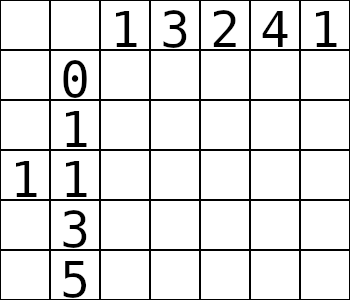
\includegraphics[width=\textwidth]{images/nonogram_example_empty.png}
        \caption{plansza przed rozwiązaniem}
    \end{subfigure}
    \begin{subfigure}[b]{0.3\textwidth}
        \centering
        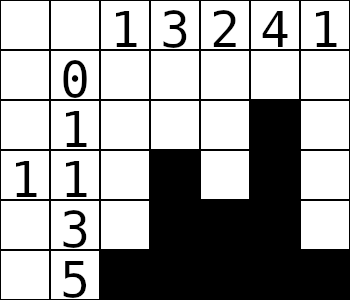
\includegraphics[width=\textwidth]{images/nonogram_example_filled.png}
        \caption{plansza po rozwiązaniu}
    \end{subfigure}
    \caption{Przykładowa plansza}
\end{figure}


\subsection{Definicje}
\begin{definition}
    Blok wypełnionych komórek w linii tworzy grupa wszystkich wypełnionych komórek z rzędu,
nieoddzielonych żadną pustą komórką.
\end{definition}
\begin{definition}
    Wskazówką nazywamy ciąg $(H_k) = (h_1, h_2, \ldots h_k)$ liczb, które opisują długości kolejnych
bloków dla danej linii.
\end{definition}
\begin{remark}
    Dla uproszczenia opisu algorytmów następuje założenie, że pusta linia jest opisywana przez
wskazówkę będącą ciągiem pustym.
\end{remark}
\begin{definition}
    Instancją problemu nonogramu jest czwórka $N = \big(w, h, (R_h), (C_w)\big)$, gdzie $w$ i $h$ 
to odpowiednio szerokość i wysokość planszy, a 
$(R_h) = \big((H_{r_1}), (H_{r_2}), \ldots, (H_{r_h})\big)$ i  
$(C_w) = \big((H_{c_1}), (H_{c_2}), \ldots, (H_{c_w})\big)$
są ciągami wskazówek dla wierszy oraz kolumn.
\end{definition}



\section{Wymagane zagadnienia matematyczne}


\begin{definition}[Problem decyzyjny]
    Problem decyzyjny to problem, na który odpowiedź stanowi 'tak' lub 'nie'.
\end{definition}
    Problem decyzyjny to pojęcie kluczowe dla klasyfikacji problemu do wybranej klasy złożoności.
By móc sklasyfikować wybrany problem (np. rozwiązanie nonogramu) do jakiejś klasy złożoności,
należy przedstawić go w postaci problemu decyzyjnego.
\begin{example}
    Czy zadany nonogram $N = \big(w, h, (R_h), (C_w)\big)$ ma rozwiązanie?
\end{example}


\begin{definition}[Klasa złożoności P]
    Klasa złożoności P zawiera wszystkie problemy decyzyjne, których rozwiązanie można znaleźć w czasie wielomianowym.
\end{definition}
\begin{example}
    Znalezienie najkrótszej ścieżki między dwoma punktami w grafie należy do klasy P, ponieważ
algorytm Dijkstry znajduje najkrótszą ścieżkę w czasie wielomianowym. Sformułowanie tego problemu
w postaci problemu decyzyjnego mogłoby brzmieć następująco: Czy dla danego wejściowego grafu $G = (V, E)$
istnieje ścieżka z punktu $v_1 \in V$ do punktu $v_2 \in V$ o długości nie większej niż $x$?
\end{example}


\begin{definition}[Klasa złożoności NP]
    Klasa złożoności NP zawiera wszystkie problemy decyzyjne, których rozwiązanie dla odpowiedzi pozytywnej
można zweryfikować w czasie wielomianowym.
\end{definition}
\begin{example}
    Mając zbiór $I$ przedmiotów, gdzie przedmiot $i_n$ to dwójka $(v_n, w_n)$, gdzie $v_n$ to wartość,
a $w_n$ to waga, oraz ograniczenie górne na sumę wag wybranych przedmiotów $w_{max}$, czy można
wybrać przedmioty w taki sposób, by nie przekroczyć limitu wagi $w_{max}$, a by suma wartości
wybranych przedmiotów była większa lub równa $c$?

    Tak zadany problem to wersja decyzyjna problemu plecakowego. Być może nie istnieje algorytm znajdujący
przydział przedmiotów w czasie wielomianowym, ale mając przedstawione rozwiązanie $S \subseteq I$
można zsumować wartości przedmiotów z $S$ i sprawdzić, czy jest to poprawne rozwiązanie.
\end{example}

    Należy zauważyć, że każdy problem z klasy \textit{P} należy także do klasy \textit{NP}, ponieważ
rozwiązanie problemu decyzyjnego jest jednym ze sposobów weryfikacji poprawności jego rozwiązania.
To czy $P = NP$ jest jak do tej pory nierozwiązanym problemem i stanowi jeden z problemów milenijnych.


\begin{definition}[Redykcja wielomianowa]
    Problem A jest redukowalny do problemu B w czasie wielomianowym, jeśli wejścia dla problemu A
można przekształcić na wejścia dla problemu B w czasie wielomianowym, a następnie rozwiązać problem A
wywołując procedurę rozwiązującą problem B wielomianową liczbę razy.
\end{definition}
\begin{example}
    Mnożenie liczb $a \cdot b$ można zdefiniować za pomocą operacji dodawania w następujący sposób:
$$a \cdot b = \underbrace{a + a + \ldots + a}_{b}$$
\end{example}
    Należy zauważyć, że jeśli problem \textit{A} jest redukowalny do problemu \textit{B} w czasie wielomianowym,
a problem \textit{B} należy do klasy P, to problem \textit{A} także należy do klasy P, jako że
sposobem na jego rozwiązanie jest użycie redukcji wielomianowej, by traktować go jako instancję problemu \textit{B},
a następnie rozwiązanie go za pomocą algorytmu działającego w czasie wielomianowym.
\begin{corollary}
    Jeśli istnieje redukcja z \textit{A} w \textit{B} w czasie wielomianowym, to \textit{B} jest
co najmniej tak złożony, jak \textit{A}.
\end{corollary}


\begin{definition}[Klasa problemów NP-trudnych]
    Problem \textit{H} należy do klasy problemów NP-trudnych, jeśli każdy problem w klasie NP 
jest redukowalny do \textit{H} w czasie wielomianowym.
\end{definition}
    W przypadku klasy problemów NP-trudnych nie ma wymogu, by należące do niej problemy były
problemami decyzyjnymi.
\begin{example}
    Przykładem problemu NP-trudnego jest problem spełnialności (SAT): 'Czy dla danej formuły logicznej
istnieje wartościowanie, dla którego zadana formuła jest spełniona?'. Przynależność tego problemu
do tej klasy została udowodniona w 1971 roku przez Stephena Cooka i Leonida Levina w dowodzie
twierdzenia Cooka-Levina \cite{Cook-Levin}.
\end{example}
    Dla udowadniania przynależności problemu do tej klasy kluczowa jest obserwacja, że istnienie
redukcji wielomianowej z \textit{A} w \textit{B} implikuje przynależność \textit{B} do tej klasy,
o ile \textit{A} także do niej należy.


\begin{definition}[Klasa problemów NP-zupełnych]
    Problem decyzyjny \textit{C} należy do klasy problemów NP-zupełnych, jeśli należy do klas problemów
NP-trudnych oraz NP.
\end{definition}
\begin{corollary}
    Pokazanie, że problem decyzyjny \textit{A} jest NP-zupełny sprowadza się do pokazania, że istnieje redukcja
wielomianowa z problemu \textit{H} z klasy problemów NP-trudnych oraz że rozwiązanie problemu \textit{A}
można zweryfikować w czasie wielomianowym.
\end{corollary}



\section{Przypisanie problemu rozwiązania nonogramów do odpowiedniej klasy złożoności}

    Mając zdefiniowane pojęcia potrzebne do klasyfikacji problemu do odpowiedniej klasy złożoności,
należy znaleźć klasę, do jakiej należy rozwiązywanie nonogramów. Z uwagi na specyfikę klas, klasyfikacji
poddana zostanie decyzyjna wersja problemu, tj. 
'\textit{Czy zadany nonogram $N = \big(w, h, (R_h), (C_w)\big)$ ma rozwiązanie?}'.


\begin{theorem}
    Problem rozwiązania nonogramu jest w NP
\end{theorem}
    Niech $M_{h, w}$ będzie macierzą oznaczająca rozwiązanie zadanego nonogramu $N = \big(w, h, (R_h), (C_w)\big)$,
gdzie $m_{i, j}$ oznacza stan komórki w wierszu $i$ i kolumnie $j$, oraz $m_{i, j} = 1$, jeśli komórka
jest wypełniona, a $m_{i, j} = 0$, jeśli komórka jest pusta. Macierz $M_{h, w}$ jest mapowana na $h + w$ list,
będących ciągami stanów komórek w kolejnych wierszach, i kolumnach.

    Do weryfikacji rozwiązania użyjemy następującej procedury:

\begin{pseudokod}[H]
    %\SetAlTitleFnt{small}
    \SetArgSty{normalfont}
    \KwIn{Lista linii $L$, lista wskazówek $LH$, długość linii $n$}
    \KwOut{Poprawność rozwiązania w osi (\texttt{true/false})}
    \For{$i \leftarrow 1$ \KwTo $|L|$}{
        $Li \leftarrow L[i]$\;
        $Hi \leftarrow LH[i]$\;
        $a \leftarrow 0$\;
        $A \leftarrow []$\;
        \For{$c \in Li$} {
            \If{$c = 1$} {
                $a \leftarrow a + 1$\;
            }
            \Else{
                \If{$a > 0$} {
                    $A.push(a)$\;
                    $a \leftarrow 0$\;
                }
            }
        }
        \If{$a > 0$} {
            $A.push(a)$\;
        }
        \For{$j \leftarrow 1 \KwTo |Hi|$} {
            \If{$A[j] \neq Hi[j]$} {
                \texttt{return false}\;
            }
        }
    }
    \texttt{return true}\;
    \caption{Poprawność rozwiązania w osi}\label{alg:axisValidation}
\end{pseudokod}

    W procedurze \ref{alg:axisValidation} następuje weryfikacja rozwiązania w danej osi. Przykładowo,
wywołując procedurę \ref{alg:axisValidation} dla listy wierszy i ich wskazówek, weryfikujemy Poprawność
rozwiązania w poziomie. Weryfikacja rozwiązania następuje przez wywołanie procedury dwukrotnie,
dla wierszy oraz kolumn. Jeśli w obu przypadkach procedura zwróci \texttt{true}, to rozwiązanie jest poprawne.

    Czas wykonania procedury jest zależny od wielkości planszy. Zewnętrzna pętla wykonuje się
tyle razy, ile jest linii w osi ($h$ w przypadku wierszy, $w$ w przypadku kolumn). Na początku pętli
dochodzi do ekstrakcji pewnych danych do lokalnych zmiennych oraz inicjalizacji tablicy - w zależności
od języka użytego do implementacji, ta grupa operacji zajmuje czas stały bądź liniowy. Następnie
uruchamiana jest pierwsza wewnętrzna pętla. W tej pętli analizowane są dane w danej linii, by zmapować
układ jej komórek do wskazówki, jaką reprezentuje. Złożoność operacji w każdej iteracji jest stała,
jeśli założymy, że powiększenie tablicy o dodatkowy element wymaga stałego czasu - w p.p. czas wykonania
iteracji może być liniowy. Liczba wykonań tej pętli zależy od długości linii.
Po wykonaniu pierwszej pętli, w zależności od układu stanu komórek w linii,
może dojść do kolejnego powiększenia tablicy o dodatkowy element - złożoność nie przekracza liniowej.
Na końcu zewnętrznej pętli wykonywana jest druga pętla, która iteruje po elementach wskazówki zadanej
w rozwiązaniu, i porównuje ich wartość do analogicznych elementów we wskazówce odtworzonej z układu linii.
Rozbieżność oznacza, że rozwiązanie nie jest prawidłowe, i procedura przedwcześnie zakańcza wykonanie.
Długość wskazówki można z góry ograniczyć przez $\lceil \frac{x}{2} \rceil$, gdzie $x$ jest długością
linii.

    Zadana procedura sprawdza poprawność rozwiązania nonogramów, a jej złożoność, w zależności od
implementacji operacji na tablicach, może wynosić $\mathcal{O}(n^2)$ bądź $\mathcal{O}(n^3)$.
Zaproponowana procedura ma złożoność wielomianową, zatem problem decyzyjny rozwiązywania nonogramów
należy do klasy \textit{NP}.


\begin{theorem}
    Problem rozwiązania nonogramu jest NP-trudny
\end{theorem}
    Dowód NP-trudności rozwiązywania nonogramów jest obszerny i wykracza poza zakres tej pracy.
Przykładowy dowód jest opisany w pracy \cite{Nonograms-NP-Hard} i jego zarys jest następujący.
Autor rozpoczyna dowód od powołania się na NP-trudność gry na grafach, nazwanej jako
\textit{Bounded Nondeterministic Constraint Logic}. Następnie, poprzez redukcję, autor udowadnia 
NP-trudność zmodyfikowanej wersji gry, określonej na grafach planarnych. Po udowodnieniu tego faktu
autor konstruuje redukcję wielomianową z planarnej \textit{Bounded Nondeterministic Constraint Logic}
w rozwiązywanie nonogramów, tym samym udowadniając ich przynależność do tej klasy problemów.


\begin{theorem}
    Problem rozwiązania nonogramu jest NP-zupełny
\end{theorem}
    Problem rozwiązania nonogramu został zaklasyfikowany do klasy problemów NP, oraz klasy problemów
NP-trudnych. Wobec tego, rozważany problem należy do klasy problemów NP-zupełnych.

	\cleardoublepage

	\chapter{Projekt systemu}
\thispagestyle{chapterBeginStyle}

    W tej części opisane zostały wymagania dla aplikacji w kontekście możliwości interakcji przez
użytkownika.



\section{Wymagania aplikacji}
\begin{enumerate}
    \item Użytkownik może wybrać jedną z predefiniowanych paczek łamigłówek by przejść do wyboru łamigłówki
    \item Użytkownik może wybrać jedną z predefiniowanych łamigłówek w paczce by przejść do jej rozwiązywania
    \item Użytkownik może rozwiązać łamigłówkę przy użyciu wyświetlanej planszy
    \item Użytkownik może oznaczać pola, co do których ma pewność, że są puste
    \item Aplikacja śledzi błędy użytkownika w trakcie rozwiązywania łamigłówki i przerywa jej rozwiązywanie
w przypadku popełnienia zbyt wielu błędów
    \item Postęp rozwiązywania łamigłówki jest zapisywany przy wyjściu do poprzedniego ekranu
    \item W menu wyboru łamigłówki wyświetlany jest stan łamigłówki tak, by można było ocenić:
    \begin{itemize}
        \item czy została rozpoczęta
        \item czy została ukończona bez przegranej
        \item czy została ukończona z przegraną
    \end{itemize}
    \item Użytkownik może wprowadzić łamigłówkę dla solvera za pomocą ekranu wprowadzania łamigłówki
    \item Użytkownik może wybrać łamigłówkę do rozwiązania dla solvera
    \item Użytkownik może nakazać rozwiązanie wprowadzonej łamigłówki
\end{enumerate}



\section{Nawigacja pomiędzy aktywnościami}
    Aplikacja otwiera się w menu głównym. W menu głównym dostępne są dwie zakładki: zakłada użytkownika
i zakładka w solvera. W zakładce użytkownika, użytkownik najpierw wybiera paczkę łamigłówek, a
następnie łamigłówkę do rozwiązania, po czym przechodzi do ekranu rozwiązywania. W zakładce solvera
dostępna jest lista wprowadzonych i predefiniowanych łamigłówek dla solvera. Użytkownik może przejść
do ekranu wprowadzania łamigłówki, by dodać kolejną łamigłówkę, bądź do ekranu auto-rozwiązywania,
gdzie nakazuje solverowi rozwiązanie wprowadzonej łamigłówki.

    Zależności między opisanymi aktywnościami są ukazane na diagramie.

\begin{figure}[!htb]
    \centering
    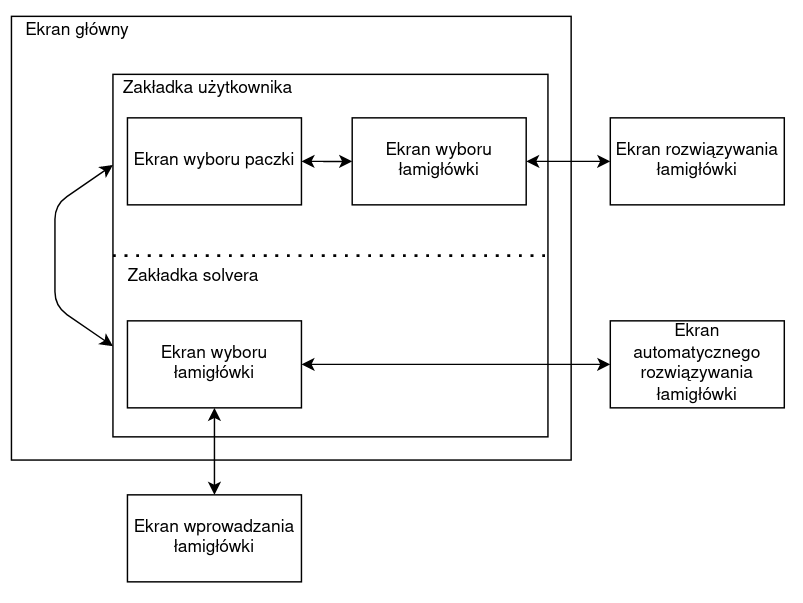
\includegraphics[width=\textwidth]{images/screens_diagram.png}
    \caption{Diagram zależności między aktywnościami}
    \label{diagAktywnosci}
\end{figure}

	\cleardoublepage
	
	\chapter{Implementacja systemu}
\thispagestyle{chapterBeginStyle}

\section{Opis technologii}

Należy tutaj zamieścić krótki opis (z referencjami) do technologii użytych przy implementacji systemu.

{\color{dgray}
Do implementacji systemu użyto języka JAVA w wersji \ldots, szczegółowy opis można znaleźć w \cite{Java}. Interfejs zaprojektowano w oparciu o HTML5 i CSS3 \cite{HTML-CSS}.
}

\section{Omówienie kodów źródłowych}

{\color{dgray}
Kod źródłowy~\ref{ws} przedstawia opisy poszczególnych metod interfejsu: \texttt{WSPodmiotRejestracjaIF}. Kompletne
kody źródłowe znajdują się na płycie CD dołączonej do niniejszej pracy w katalogu \texttt{Kody} (patrz Dodatek~\ref{plytaCD}).
}

\begin{small}
\begin{lstlisting}[language=Java, frame=lines, numberstyle=\tiny, stepnumber=5, caption=Interfejs usługi Web Service: \texttt{WSPodmiotRejestracjaIF}\label{ws}., firstnumber=1]
package erejestracja.podmiot;
import java.rmi.RemoteException;
// Interfejs web serwisu dotyczącego obsługi podmiotów i rejestracji.
public interface WSPodmiotRejestracjaIF extends java.rmi.Remote{
// Pokazuje informacje o danym podmiocie.
// parametr: nrPeselRegon - numer PESEL podmiotu lub numer REGON firmy.
// return: Podmiot - obiekt transportowy: informacje o danym podmiocie.
public Podmiot pokazPodmiot(long nrPeselRegon) throws RemoteException;
// Dodaje nowy podmiot.
// parametr: nowyPodmiot - obiekt transportowy: informacje o nowym podmiocie.
// return: true - jeśli podmiot dodano, false - jeśli nie dodano.
public boolean dodajPodmiot(Podmiot nowyPodmiot) throws RemoteException;
// Usuwa dany podmiot.
// parametr: nrPeselRegon - numer PESEL osoby fizycznej lub numer REGON firmy.
// return: true - jeśli podmiot usunięto, false - jeśli nie usunięto.
public boolean usunPodmiot(long nrPeselRegon) throws RemoteException;
// Modyfikuje dany podmiot.
// parametr: podmiot - obiekt transportowy: informacje o modyfikowanym podmiocie.
// return: true - jeśli podmiot zmodyfikowano, false - jeśli nie zmodyfikowano.
public boolean modyfikujPodmiot(Podmiot podmiot) throws RemoteException;
// Pokazuje zarejestrowane podmioty na dany dowód rejestracyjny.
// parametr: nrDowoduRejestracyjnego - numer dowodu rejestracyjnego.
// return: PodmiotRejestracja[] - tablica obiektów transportowych: informacje o
// wszystkich zarejestrowanych podmiotach.
public PodmiotRejestracja[] pokazZarejestrowanePodmioty(
String nrDowoduRejestracyjnego) throws RemoteException;
// Nowa rejestracja podmiotu na dany dowód rejestracyjny.
// parametr: nrDowoduRejestracyjnego - numer dowodu rejestracyjnego.
// parametr: nrPeselRegon - numer PESEL podmiotu lub numer REGON firmy.
// parametr: czyWlasciciel - czy dany podmiot jest właścicielem pojazdu.
// return: true - jeśli zarejestrowano podmiot, false - jeśli nie zarejestrowano.
public boolean zarejestrujNowyPodmiot(String nrDowoduRejestracyjnego,
long nrPeselRegon, boolean czyWlasciciel) throws RemoteException;
// Usuwa wiązanie pomiędzy danym podmiotem, a dowodem rejestracyjnym.
// parametr: nrDowoduRejestracyjnego - numer dowodu rejestracyjnego.
// parametr: nrPeselRegon - numer PESEL podmiotu lub numer REGON firmy.
// return: true - jeśli podmiot wyrejestrowano, false - jeśli nie wyrejestrowano.
public boolean wyrejestrujPodmiot(String nrDowoduRejestracyjnego,
long nrPeselRegon) throws RemoteException;
\end{lstlisting} 
\end{small}

{\color{dgray}
Kod źródłowy~\ref{req} przedstawia procedurę przetwarzającą żądanie. Hasz utrwalany \verb|%granulacja| wykorzystywany jest do komunikacji międzyprocesowej.
}

\begin{small}
\begin{lstlisting}[language=perl, frame=lines, caption=Przetwarzanie żądania - procedura \texttt{process\_req()}\label{req}., firstnumber=86]
sub process_req(){	
  my($r) = @_;
  $wyn = "";
  if ($r=~/get/i) {
	@reqest = split(" ",$r);
	$zad = $reqest[0];
	$ts1 = $reqest[1];
	$ts2 = $reqest[2];
	@date1 = split(/\D/,$ts1);
	@date2 = split(/\D/,$ts2);
	print "odebralem: $r"; 
	$wyn = $wyn."zadanie: $zad\n";
	$wyn = $wyn."czas_od: "."$date1[0]"."-"."$date1[1]"."-"."$date1[2]"."_"."$date1[3]".":"."$date1[4]".":"."$date1[5]"."\n";
	$wyn = $wyn."czas_do: "."$date2[0]"."-"."$date2[1]"."-"."$date2[2]"."_"."$date2[3]".":"."$date2[4]".":"."$date2[5]"."\n";		
	$wyn = $wyn.&sym_sens($ts1,$ts2);
	return $wyn;
  }
  if ($r=~/set gt/i) {
	@reqest = split(" ",$r);
	$zad = $reqest[0];
	$ts1 = $reqest[1];
	$ts2 = $reqest[2];
	$gt = $reqest[2];
	dbmopen(%granulacja,"granulacja_baza",0644);
	$granulacja{"gt"}=$gt;
	dbmclose(%granulacja);
	$wyn = "\'GT\' zmienione na: $gt";
  }		
}	
\end{lstlisting} 
\end{small}

	\cleardoublepage
	
	\chapter{Solver nonogramów}
\thispagestyle{chapterBeginStyle}

    W tym rozdziale opisany jest rozwój solvera. Opisane są kolejne główne wersje solverów, zbadany
jest także wpływ zastosowanych heurystyk na wydajność w rozwiązywaniu wybranych łamigłówek.



\section{Wersje solverów}


\subsection{Solver całościowy}
    Solver całościowy jest najprostszym z solverów implementowanych w toku pisania aplikacji. Jego
implementacja opiera się na założeniu, że obrazek ukryty w łamigłówce jest ciągiem pustych i pełnych
pikseli. Solver sprawdza wszystkie możliwe kombinacje pól, aż do wykrycia rozwiązania, bądź stwierdzenia
jego braku. Wskazówki umieszczone obok planszy służą jedynie do walidacji rozwiązania, i nie są
wykorzystywane w trakcie rozwiązywania nonogramu.

\begin{figure}[!htb]
    \centering
    
\includegraphics[width=0.5\textwidth]{images/all_solver_example.png}
    \caption{Solver całościowy sprawdza wszystkie możliwe układy planszy w celu znalezienia rozwiązania.}
\end{figure}

    Solver ten zaczyna od pustej planszy. Następnie, dla pierwszego pola wywoływana jest rekursyjna
metoda: jeśli indeks pola mieści się w zakresie planszy, to najpierw jego status ustawiany jest na
pusty, i następuje wywołanie metody dla nastepnego indeksu, a jeśli rozwiązanie nie zostanie znalezione,
to pole jest wypełniane i ponownie dochodzi do wywołania metody na następnym polu. Jeśli indeks
wykracza poza zakres planszy, to znaczy że wszystkie pola mają ustawiony status i wywoływana jest
metoda sprawdzająca poprawność rozwiązania, podobna do tej opisanej w \ref{alg:axisValidation}.
Jeśli solver zakończy działanie zwracając \texttt{true}, to w przekazanej mu macierzy pól 
(równoznaczne z listą wierszy) znajdzie się rozwiązanie łamigłówki.

\begin{pseudokod}[H]
    %\SetAlTitleFnt{small}
    \SetArgSty{normalfont}
    \SetKwFunction{Verify}{Verify}
    \KwIn{Lista wierszy $R$, indeks pola $i$, lista wskazówek wierszy $Hr$ i kolumn $Hc$, szerokość $w$ i wysokość $h$ planszy}
    \KwOut{Czy znaleziono rozwiązanie \texttt{true/false}}
    \If{$i \geq w \cdot h$}{
        \texttt{return} \Verify{$R$, $Hr$, $Hc$, $w$, $h$}\;
    }
    \Else{
        $iWiersza \leftarrow \lceil \frac{i}{w} \rceil$\;
        $iKolumny \leftarrow i\ mod\ w$\;
        $R[iWiersza][iKolumny] \leftarrow 0$\;
        \If{\texttt{SolverCałościowy}($R, i+1, Hr, Hc, w, h$)}{
            \texttt{return true}\;
        }
        $R[iWiersza][iKolumny] \leftarrow 1$\;
        \texttt{return SolverCałościowy}($R, i+1, Hr, Hc, w, h$)\;
    }
    \caption{SolverCałościowy}\label{alg:allSolver}
\end{pseudokod}

    Złożoność czasowa tego solvera jest bardzo duża. Procedura sprawdzająca poprawność rozwiązania
może zostać wywołana $2^{w*h}$ razy, czyli inaczej $2^n$, gdzie $n$ to ilość pól na planszy. 
Wynika to z faktu, że kazde kolejne pole wymaga sprawdzenia pól poprzednich, a samo może znajdować
się w dwóch stanach, więc podwaja ilość wywołań procedury sprawdzającej.


\subsection{Solver osiowy}
    W odróżnieniu od solvera całościowego, solver osiowy korzysta ze wskazówek przy szukaniu rozwiązań.
Opiera się on na fakcie, że każda linia (wiersz lub kolumna) może znajdować się w jednym z możliwych
stanów, których liczba nigdy nie dojdzie do $2^x$, gdzie $x$ jest długością linii. Sprawdzając
rozwiązanie w tym solverze, gwarantowana jest poprawność w jednej z osi, co dodatkowo znacząco skraca
czas szukania rozwiązania.

\begin{figure}[!htb]
    \centering
    
\includegraphics[width=0.5\textwidth]{images/axis_solver_example.png}
    \caption{Dla linii na grafice, solver osiowy spradza jedynie 3 stany. Dla tej samej linii,
solver całościowy sprawdziłby $2^5 = 32$ stany
    }
\end{figure}

    Solver zaczyna od pustej planszy. Przed rozpoczęciem rozwiązywania sprawdzana jest ilość wszystkich
kombinacji w danej osi (iloczyn możliwości każdej z linii), i wybierana jest oś z mniejszą liczbą
możliwości. Następnie generowane są kombinacje dla każdej z linii. Solver korzysta z rekursyjnej
metody, i ustawia pierwszą kombinację dla pierwszej linii. Następnie wywołuje metodę dla kolejnej linii,
aż do ostatniej, i wtedy weryfikuje rozwiązanie. Jeśli dla danego ustawienia w linii łamigłówka
nie ma rozwiązania, to solver przechodzi do kolejnego ustawienia i wywołuje metodę w kolejnej linii.

\begin{pseudokod}[H]
    %\SetAlTitleFnt{small}
    \SetArgSty{normalfont}
    \SetKwFunction{Verify}{Verify}
    \SetKwFunction{NalozKombinacje}{NalozKombinacje}
    \KwIn{Lista linii $L$, indeks linii $i$, lista wskazówek linii prostopadłych $H$, ilość linii $n$}
    \KwOut{Czy znaleziono rozwiązanie \texttt{true/false}}
    \If{$i = n$}{
        \texttt{return} \Verify{$L$, $H$, $n$}\;
    }
    \Else{
        $linia \leftarrow L[i]$\;
        \ForEach{$komb \in linia.kombinacje$}{
            \NalozKombinacje{$linia, komb$}\;
            \If{\texttt{SolverOsiowy}($L, i+1, H, n$)}{
                \texttt{return true}\;
            }
        }
        \texttt{return false}\;
    }
    \caption{SolverOsiowy}\label{alg:axisSolver}
\end{pseudokod}

    Dzięki eliminacji kombinacji sprzecznych ze wskazówkami w danej osi, procedura sprawdzania
poprawności rozwiązania jest wywoływana o wiele rzadziej niż w przypadku solvera całościowego.
O ile ilość kombinacji w linii przy rozpatrywaniu każdej komórki z osobna to $2^n$, gdzie $n$ to
długość linii, tak w przypadku rozważania poprawnych kombinacji dla linii jest ona zależna od
długości i zawartości wskazówki, i można ją ograniczyć z góry przez
${n + 1 - h} \choose h$, a $h$ to ilość wskazówek w linii. To przybliżenie jest zawyżone, ponieważ
zakłada występowanie jedynie bloków długości jeden we wskazówce. W przeciętnym przypadku, bloki
wypełnionych komórek będą dłuższe, oraz będzie ich mniej. Dodatkowo, jak zostało wspomniane na początku,
weryfikacja jest wymagana jedynie w jednej z dwóch osi, jako że konstrukcja potencjalnych rozwiązań
opiera się o zestawianie poprawnych kombinacji z linii.


\subsection{Solver eliminacyjny}
    Solverem, którego wariant znajduje się w aplikacji, jest solver eliminacyjny. W przeciwieństwie
do wcześniej opisanych solverów, solver ten nie zakłada układów komórek w liniach tak długo jak to
możliwe. W jego wypadku, generowane są możliwe kombinacje dla każdej z linii (zarówno wierszy jak i
kolumn). W danym przejściu eliminowane są kombinacje sprzeczne z dostępnymi informacjami 
(np. kombinacje posiadające pełną pierwszą komórkę, podczas gdy pewne jest że jest ona pełna) 
oraz wyciągane są części wspólne kombinacji (np. wszystkie kombinacje mają pustą drugą komórkę), 
które dostarczają informacji dla innych linii. Dodatkowo, w przeciwieństwie do poprzednich solverów,
nie jest konieczna walidacja rozwiązania, jako że rozwiązanie jest poprawne w momencie, gdy każdy
wiersz i każda kolumna ma dostępną jedną możliwą komibnację.

\begin{figure}[!htb]
    \centering
    \begin{subfigure}[b]{0.35\textwidth}
        \centering
        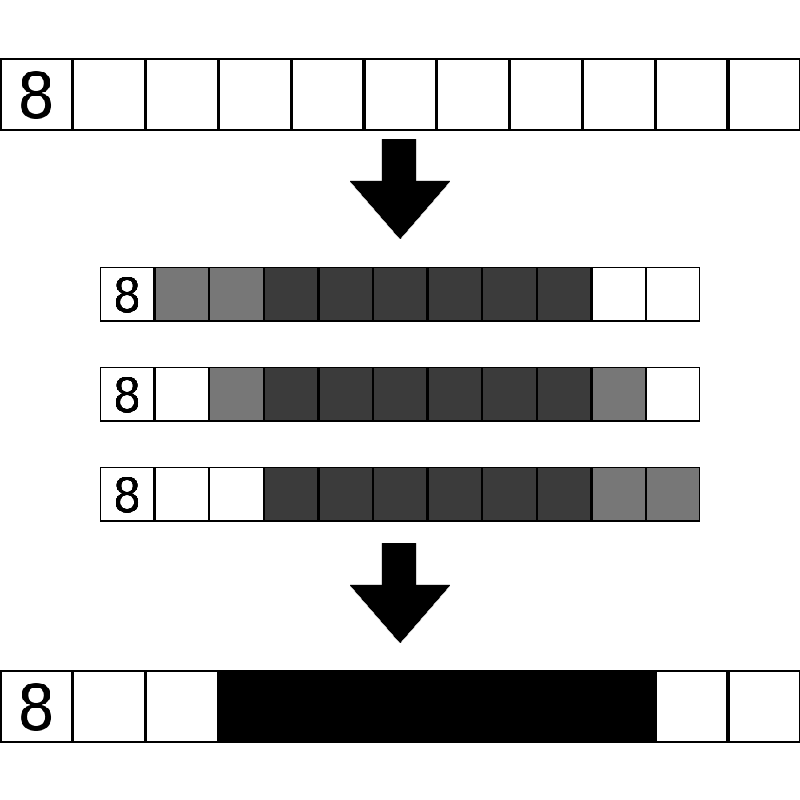
\includegraphics[width=\textwidth]{images/elimination_solver_example_a.png}
        \caption{pola wspólne dla wszystkich kombinacji zostają naniesione na planszę}
    \end{subfigure}
    \hspace{0.1\textwidth}
    \begin{subfigure}[b]{0.35\textwidth}
        \centering
        
\includegraphics[width=\textwidth]{images/elimination_solver_example_b.png}
        \caption{korzystając z informacji z wiersza, solver wnioskuje stan większości pól w kolumnie
        (x oznacza pole definitywnie puste)}
    \end{subfigure}
    \caption{Przykład wnioskowania na podstawie możliwych kombinacji}
\end{figure}

    Solver zaczyna od pustej planszy. Na początku generowane są wszystkie kombinacje dla każdej z
linii, a linie wrzucane są do kolejki \textit{last-in first-out}. Następnie solver przechodzi do
rozwiązywania. Dopóki kolejka nie jest pusta, to są linie, których komibnacje należy zweryfikować.
Z kolejki usuwana jest sprawdzana linia. Dla tej linii następują dwa kroki: najpierw, eliminowane
są kombinacje sprzeczne z układem danej linii. W wypadku tego solvera, każda komórka znajduje się
w jednym z trzech stanów: \textit{pełny}, \textit{pusty} i \textit{nieznany}. Stan \textit{nieznany}
komórki dopuszcza kombinacje zawierające komórkę pełną lub pustą; pozostałe stany wymagają
zgodności stanu ze stanem komórki w kombinacji. Po eliminacji sprzecznych kombinacji, dochodzi
do porównania kombinacji. Jeśli istnieje komórka w linii, której stan jest \textit{nieznany}, a
wszystkie pozostałe kombinacje mają ustawiony dla niej ten sam stan, to stan komórki jest aktualizowany,
a prostopadła linia zostaje dodana do kolejki do weryfikacji (następuje przy tym upewnienie, że
w kolejce nie ma powtórzeń). Kiedy kolejka zostanie opróżniona, sprawdzane są linie.
Jeśli wszystkie linie mają jeden możliwy stan, to znaczy że zostało znalezione rozwiązanie. Jeśli
któraś z linii nie ma możliwej kombinacji, to nie istnieje rozwiązanie przy dokonanych założeniach.
W przeciwnym wypadku, solver zakłada poprawność jednej z kombinacji dla linii
o kilku możliwych kombinacjach. Jako że wskutek założenia stan linii zmienił się, to do kolejki
dodawane są linie prostopadłe. Następnie wywoływana jest w sposób rekursyjny metoda rozwiązująca
nonogram dla obecnego stanu planszy. Jeśli rozwiązanie nie zostanie znalezione w tej gałęzi, to
solver zakłada poprawność kolejnej kombinacji dla tej linii.

\begin{pseudokod}[H]
    %\SetAlTitleFnt{small}
    \SetArgSty{normalfont}
    \SetKwFunction{SprawdzLinie}{SprawdzLinie}
    \SetKwFunction{NalozKombinacje}{NalozKombinacje}
    \SetKwFunction{UzupelnijKolejke}{UzupelnijKolejke}
    \KwIn{Lista wierszy $R$ i kolumn $C$, kolejka $Q$}
    \KwOut{Czy znaleziono rozwiązanie \texttt{true/false}}
    \ForEach{$linia \in Q$}{
        \SprawdzLinie{$linia$}\;
    }
    \If{$(\forall linia \in R \bigcup C)(|linia.kombinacje| = 1)$}{
        \texttt{return true}\;
    }
    \uElseIf{$(\exists linia \in R \bigcup C)(|linia.kombinacje| = 0)$}{
        \texttt{return false}\;
    }
    \Else{
        $zakladanaLinia \leftarrow$ pierwsza linia z wieloma kombinacjami\;
        \ForEach{$komb \in zakladanaLinia.kombinacje$}{
            $kopiaR \leftarrow kopiuj(R)$\;
            $kopiaC \leftarrow kopiuj(C)$\;
            \NalozKombinacje{$zakladanaLinia, komb$}\;
            \UzupelnijKolejke{$Q$}\;
            \If{\texttt{SolverEliminacyjny}($kopiaR, kopiaC, Q$)}{
                $R \leftarrow kopiaR$\;
                $C \leftarrow kopiaC$\;
                \texttt{return true}\;
            }
        }
        \texttt{return false}\;
    }
    \caption{SolverEliminacyjny}\label{alg:eliminationSolver}
\end{pseudokod}

    Istotna uwaga dotyczy charakterystyki wierszy i kolumn. W celu umożliwienia działania procedury
został wykorzystany mechanizm obecny w wielu powszechnie używanych językach programowania, mianowicie
mechanizm płytkiej kopii. Mimo że listy wierszy i kolumn zawierają inne obiekty (listy), to obiekty
komórek przechowywane w tych zagnieżdżonych listach są takie same. Dzięki temu, modyfikując stan
komórki w liście wierszy w $n$-tym wierszu i $m$-tej komórce, modyfikujemy także stan komórki
zawartej w $n$-tej komórce w $m$-tej kolumnie w liście kolumn.



\section{Porównanie wydajności solverów}
    W tej części zbadane zostały wydajności poszczególnych wersji solverów oraz wpływ wybranych
modyfikacji i heurystyk na ich wydajność.


\subsection{Metodyka badań}
    Metoda prowadzenia badań jest następująca: dla każdej łamigłówki prowadzonych jest 5 prób 
rozwiązania. Próby z minimalnym oraz maksymalnym czasem rozwiązywania zostają odrzucone, w celu
eliminacji błędów powstałych na skutek zaburzeń występujących w trakcie prowadzenia testu. Następnie
czas pozostałych 3 prób zostaje uśredniony i podany jako wynik badania. Jeśli czas wykonania
iteracji testu przekroczy 5 minut, to test zostaje przerwany i do komórki zostaje wpisany wynik
\textit{przekroczono}.

    Testy zostały przeprowadzone na komputerze z procesorem Intel Core i5-6300HQ \cite{i5-6300hq}, z
16GB pamięci RAM o taktowaniu 2133Mhz. Testy zostały uruchomione w środowisku Node.js \cite{node}
w wersji v14.18.2. Czas rozwiązywania łamigłówek na urządzeniu mobilnym może znacząco odbiegać
od czasów zaprezentowanych w wynikach, z powodu mniejszych zasobów i zastosowanego środowiska
uruchomieniowego.

    Wyniki zostały zaprezentowane w tabelach o następującym układzie: w pierwszych dwóch kolumnach
zostały podane nazwy łamigłówek i ich wielkości (łamigłówki są zadane na planszach kwadratowych).
W kolejnych kolumnach, nazwanych odpowiednio do zastosowanej modyfikacji bądź jej braku,
podany jest czas rozwiązywania nonogramu wyrażony w milisekundach. Czas jest zaokrąglony do pełnych
milisekund, zatem dla prostych łamigłówek może być wyrażony jako 0.

    Zestaw danych użyty do testów został przedstawiony na końcu rozdziału.


\subsection{Solver całościowy}
    Wydajność solvera całościowego została sprawdzona na zestawie 4 łamigłówek.

\subsubsection{Wyniki}
\begin{table}[h]
    \begin{center}
        \begin{tabular}{|c|c|r|}
            \hline
            Nazwa          & Rozmiar        & Czas rozwiązywania w ms \\
            \hline
            Cross       & 3 & 1                     \\
            Flame       & 5 & 46                    \\
            Jellyfish   & 8 & \textit{przekroczono} \\
            Candy       & 8 & \textit{przekroczono} \\
            \hline
        \end{tabular}
    \end{center}
    \caption{Wyniki testów dla solvera całościowego}
\end{table}

\subsubsection{Interpretacja}
    Solver całościowy jest w stanie dość szybko rozwiązać niewielkie łamigłówki,
ale czas jego pracy rośnie bardzo szybko wraz ze wzrostem wielkości planszy.


\subsection{Solver osiowy}
    Wydajność solvera całościowego została sprawdzona na pełnym zestawie 18 łamigłówek. Został
on poddany jednej modyfikacji.

\subsubsection{Modyfikacje}
    \textbf{Częściowa weryfikacja} rozwiązania polega na wykorzystaniu procedury częsciowej weryfikacji.
Jest ona podobna do procedury weryfikacji w osi, ale nie sprawdza poprawności całej planszy,
a jedynie sprawdza czy dany układ może prowadzić do poprawnego rozwiązania (czyli czy nie ma sprzeczności na tym etapie).
Procedura otrzymuje głębokość dla jakiej ma zweryfikować poprawność. Jeśli do danej głębokości nie
występuje sprzeczność, to rozwiązanie jest konstruowane dalej. W przeciwnym przypadku, w danej gałęzi
nie może być poprawnego rozwiązania, i solver przechodzi do innej gałęzi.

\begin{figure}[!htb]
    \centering
    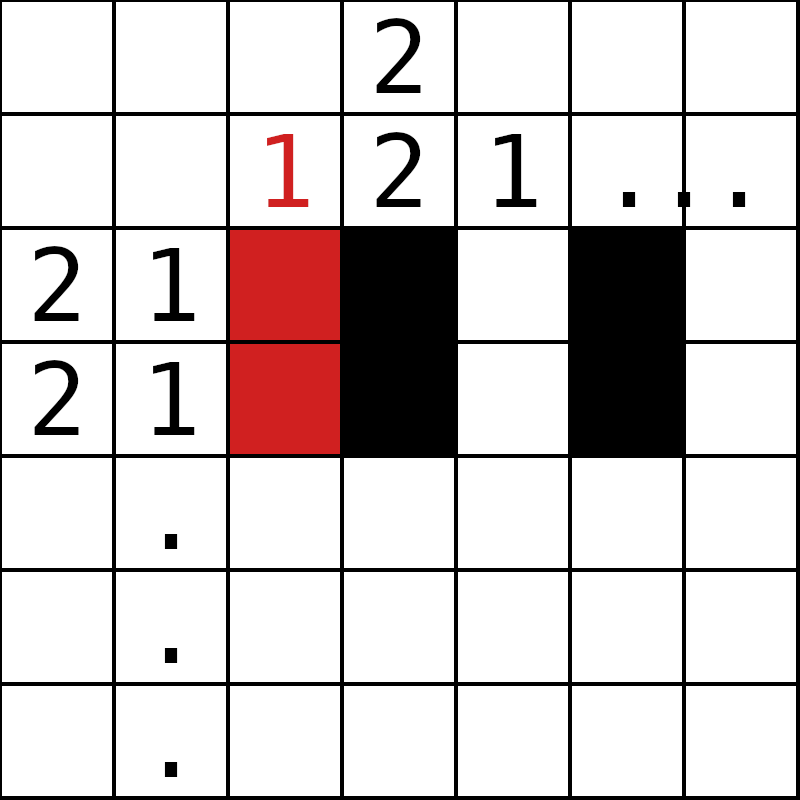
\includegraphics[width=0.4\textwidth]{images/partial_check_example.png}
    \caption{Na tym etapie można zdyskwalifikować każde rozwiązanie zawierające pierwszy i drugi wiersz
w układzie widocznym na grafice}
\end{figure}



\subsubsection{Wyniki}
\begin{table}[h!]
    \begin{center}
        \begin{tabular}{|c|c|r r|}
            \hline
            {}          & {}        & \multicolumn{2}{c|}{Czas rozwiązywania w ms} \\
            Nazwa       & Rozmiar   & bez modyfikacji & z częściową weryfikacją \\
            \hline
            Cross       & 3         & 0                     & 0 \\
            Flame       & 5         & 0                     & 0 \\
            Jellyfish   & 8         & 463                   & 2 \\
            Candy       & 8         & 0                     & 0 \\
            Shield      & 10        & \textit{przekroczono} & 3 \\
            Dog         & 10        & 12004                 & 1 \\
            Duck        & 16        & \textit{przekroczono} & 12 \\
            Shrimp      & 16        & \textit{przekroczono} & 14 \\
            Cherries    & 20        & \textit{przekroczono} & 25 \\
            Potion      & 20        & \textit{przekroczono} & 315 \\
            Tape        & 25        & \textit{przekroczono} & 1091 \\
            Lighter     & 25        & \textit{przekroczono} & 60945 \\
            \hline
            Ghost       & 32        & \textit{przekroczono} & 40040 \\
            Demon       & 32        & \textit{przekroczono} & 3997 \\
            Butcher     & 48        & \textit{przekroczono} & \textit{przekroczono} \\
            Ranger      & 48        & \textit{przekroczono} & 59703 \\
            Orc         & 64        & \textit{przekroczono} & \textit{przekroczono} \\
            Swordsman   & 64        & \textit{przekroczono} & \textit{przekroczono} \\
            \hline
        \end{tabular}
    \end{center}
    \caption{Wyniki testów dla solvera osiowego}
\end{table}

\subsubsection{Interpretacja}
    W podstawowej wersji, solver osiowy ma niewiele lepszą wydajność od solvera całościowego,
będąc w stanie rozwiązać niektóre łamigłówki wielkości 10 przy nałożonym ograniczeniu czasowym. 
Jednak po dodaniu częsciowej weryfikacji, wydajność solvera drastycznie wzrasta, i może zostać
wykorzystany do rozwiązywania łamigłówek o wiele większych niż w przypadku podstawowej wersji.
Pokazuje to jak kluczowa jest wstępna eliminacja niepożądanych gałęzi przy rozwiązywaniu danego
problemu.


\subsection{Solver eliminacyjny}
    Wydajność solvera całościowego została sprawdzona na pełnym zestawie 18 łamigłówek.

\subsubsection{Modyfikacje}
    \textbf{Rozwiązywanie bez przerywania} (\textit{bez przerw.}) to modyfikacja polegająca na
usunięciu warunkowego przerwania szukania rozwiązania. Zamiast przerwać w momencie znalezienia
kolumny nie zawierającej żadnej poprawnej kombinacji, solver szuka dalej, aż do opróżnienia kolejki,
i dopiero wtedy informuje o braku rozwiązania. Z uwagi na częste korzystanie z kolejki, eliminacja
tej instrukcji mogłaby skrócić czas wykonywania jednego sprawdzenia linii.

    \textbf{Zakładanie dla kolumn} (\textit{kolumny}) zmienia kolejność zakładania. Linia z wieloma
kombinacjami jest szukana najpierw na liście kolumn, a dopiero potem na liście wierszy. Ta modyfikacja
opiera się na założeniu, że układ wypełnionych pól w łamigłówkach powoduje lepszą wydajność
przy rozwiązywaniu pionowym.

    \textbf{Zakładanie dla linii z minimalną/maksymalną liczbą kombinacji} (\textit{min/max komb.})
dokonuje założenia dla linii z najmniejszą/największą liczbą poprawnych kombinacji. W ten sposób
badany jest wpływ doboru sposobu zakładania na czas szukania rozwiązania.

    \textbf{Kolejność linii w kolejce} to seria modyfikacji sprawdzających wpływ typu kolejki
na czas rozwiązania. W kolumnie \textit{lifo} podane są wyniki dla kolejki, w której nowo dodane
bądź ponownie dodane linie są przesuwane na początek kolejki. W \textit{fifo} przedmioty są wrzucane
na koniec kolejki. \textit{bez zm.} oznacza, że przedmioty są ustawiane na początku kolejki, ale
ponowne dodanie nie zmienia kolejności przedmiotów w kolejce. W kolejnych trzech kolumnach
(\textit{śl. ind. lifo}, \textit{śl. ind. fifo}, \textit{śl. ind. bez zm.}) badane są te same
własności kolejki, ale struktura ta zostaje zmodyfikowana tak, by śledzić linie wraz ze zmodyfikowanymi
indeksami. Dzięki temu nie jest konieczne sprawdzenie każdego indeksu w linii, a jedynie tych komórek
dla których zaszła zmiana.


\subsubsection{Wyniki}

\begin{table}[h!]
    \begin{center}
        \begin{tabular}{|c|c|r r r r r|}
            \hline
            {}          & {}        & \multicolumn{5}{c|}{Czas rozwiązywania w ms} \\
            Nazwa       & Rozmiar   & bez modyfikacji & bez przerw. & kolumny & min komb. & max komb. \\
            \hline
            Cross       & 3         & 0     & 0     & 0     & 0     & 0     \\
            Flame       & 5         & 0     & 0     & 0     & 0     & 0     \\
            Jellyfish   & 8         & 1     & 1     & 1     & 1     & 1     \\
            Candy       & 8         & 0     & 0     & 0     & 0     & 0     \\
            Shield      & 10        & 2     & 2     & 2     & 2     & 1     \\
            Dog         & 10        & 1     & 0     & 0     & 0     & 1     \\
            Duck        & 16        & 2     & 1     & 1     & 1     & 1     \\
            Shrimp      & 16        & 1     & 1     & 1     & 1     & 1     \\
            Cherries    & 20        & 3     & 3     & 3     & 3     & 3     \\
            Potion      & 20        & 12    & 13    & 13    & 13    & 13    \\
            Tape        & 25        & 2     & 2     & 2     & 2     & 2     \\
            Lighter     & 25        & 13    & 13    & 13    & 12    & 13    \\
            \hline
            Ghost       & 32        & 47    & 47    & 48    & 45    & 47    \\
            Demon       & 32        & 1787  & 1817  & 1806  & 1800  & 1822  \\
            Butcher     & 48        & 1811  & 1809  & 1819  & 1790  & 1791  \\
            Ranger      & 48        & 46    & 48    & 47    & 47    & 48    \\
            Orc         & 64        & 1463  & 1454  & 1446  & 1465  & 1456  \\
            Swordsman   & 64        & 1440  & 1467  & 1451  & 1429  & 1432  \\
            \hline
        \end{tabular}
    \end{center}
    \caption{I część wyników dla solvera eliminacyjnego}
\end{table}

\begin{table}[h]
    \begin{center}
        \begin{tabular}{|c|c|r r r r r r|}
            \hline
            {}          & {}        & \multicolumn{6}{c|}{Czas rozwiązywania w ms} \\
            Nazwa       & Rozmiar   & lifo & fifo & bez zm. & śl. ind. lifo & śl. ind. fifo & śl. ind. bez zm. \\
            \hline
            Cross       & 3         & 0     & 0     & 0     & 0     & 0     & 0     \\
            Flame       & 5         & 0     & 0     & 0     & 0     & 0     & 0     \\
            Jellyfish   & 8         & 1     & 2     & 2     & 2     & 1     & 1     \\
            Candy       & 8         & 0     & 0     & 0     & 0     & 0     & 0     \\
            Shield      & 10        & 2     & 1     & 1     & 2     & 3     & 2     \\
            Dog         & 10        & 1     & 1     & 1     & 1     & 0     & 1     \\
            Duck        & 16        & 2     & 1     & 2     & 2     & 2     & 2     \\
            Shrimp      & 16        & 1     & 1     & 1     & 1     & 1     & 1     \\
            Cherries    & 20        & 3     & 4     & 4     & 3     & 4     & 3     \\
            Potion      & 20        & 12    & 13    & 14    & 16    & 16    & 13    \\
            Tape        & 25        & 2     & 2     & 2     & 4     & 3     & 3     \\
            Lighter     & 25        & 13    & 13    & 13    & 13    & 15    & 13    \\
            \hline
            Ghost       & 32        & 47    & 47    & 52    & 56    & 72    & 54    \\
            Demon       & 32        & 1787  & 2380  & 1980  & 1194  & 1257  & 1127  \\
            Butcher     & 48        & 1811  & 1884  & 1798  & 1854  & 1962  & 1717  \\
            Ranger      & 48        & 46    & 44    & 53    & 61    & 62    & 59    \\
            Orc         & 64        & 1463  & 1413  & 1437  & 1413  & 1415  & 1311  \\
            Swordsman   & 64        & 1440  & 1489  & 1544  & 1534  & 1608  & 1451  \\
            \hline
        \end{tabular}
    \end{center}
    \caption{II część wyników dla solvera eliminacyjnego}
\end{table}

\subsubsection{Interpretacja}
    Solver eliminacyjny jest najszybszym z zaprezentowanych solverów. Jest w stanie rozwiązać
nawet największe, 64x64 nonogramy w założonym ograniczeniu czasowym. Każdą ze sprawdzanych łamigłówek
rozwiązuje szybciej niż solver osiowy. Na szczególną uwagę zasługuje szybkość rozwiązania nonogramów
\textit{Ghost} i \textit{Ranger}. Dzięki oparciu się o informacje wywnioskowane z poprzednio
rozpatrywanych linii, solver może rozwiązać nawet łamigłówki o dużych rozmiarach bez zakładania
układu linii, lub z minimalną jego ilością.

    Pierwsza seria modyfikacji nie miała dużego wpływu na czas rozwiązywania. W drugiej serii
modyfikacji, niektóre modyfikacje okazały się kluczowe dla czasu działania. Użycie kolejki
typu \textit{first-in first-out} z przerzucaniem na koniec przy aktualizacji linii znacznie spowolniło
czas rozwiązywania łamigłówki \textit{Demon} w przypadku bazowej wersji solvera,
a w przypadku wersji ze śledzeniem indeksów różnica była mniejsza, ale zauważalna.
Oprócz tego, modyfikacja struktury danych w celu śledzenia modyfikowanych indeksów
okazała się dobrym pomysłem, jako że solver korzystający z niej (\textit{śl. ind. bez zm.}) osiągnął
najlepsze czasy dla trudniejszych łamigłówek (np. \textit{Demon}, \textit{Butcher}), 
będąc nieznacznie wolniejszym dla łamigłówek prostszych (np. \textit{Ghost}, \textit{Ranger}).


\subsection{Wnioski}
    Solver eliminacyjny jest najwydajniejszym z zaproponowanych solverów. Dzięki oparciu na pewnych
informacjach i ograniczeniu zakładania, a co za tym idzie back-trackingu, może rozwiązać zadaną
łamigłówkę szybbiej niż inne solvery. W przypadku solvera osiowego, introdukcja częściowej weryfikacji
bardzo poprawiła jego wydajność.


\subsection{Zestaw danych}
    Do przeprowadzenia badań zostały użyte następujące obrazy, które po konwersji zostały przekazane do solverów
jako zestaw wskazówek. Grafiki zawierające kolor biały zostały nałożone na tło w kolorze magenta
w celu wyróżnienia tego koloru na tle białej kartki.

\begin{figure}[!htb]
    \centering
    \begin{subfigure}[b]{0.1\textwidth}
        \centering
        
\includegraphics[width=\textwidth]{images/data_set/3x3_cross.png}
        \caption{Cross}
    \end{subfigure}
    \begin{subfigure}[b]{0.1\textwidth}
        \centering
        
\includegraphics[width=\textwidth]{images/data_set/5x5_flame.png}
        \caption{Flame}
    \end{subfigure}
    \begin{subfigure}[b]{0.1\textwidth}
        \centering
        
\includegraphics[width=\textwidth]{images/data_set/8x8_jellyfish.png}
        \caption{Jellyfish \cite{8x8-src}}
    \end{subfigure}
    \begin{subfigure}[b]{0.1\textwidth}
        \centering
        
\includegraphics[width=\textwidth]{images/data_set/8x8_candy.png}
        \caption{Candy \cite{8x8-src}}
    \end{subfigure}
    \begin{subfigure}[b]{0.1\textwidth}
        \centering
        
\includegraphics[width=\textwidth]{images/data_set/10x10_shield.png}
        \caption{Shield \cite{10x10-src}}
    \end{subfigure}
    \begin{subfigure}[b]{0.1\textwidth}
        \centering
        
\includegraphics[width=\textwidth]{images/data_set/10x10_dog.png}
        \caption{Dog \cite{10x10-src}}
    \end{subfigure}
    \begin{subfigure}[b]{0.1\textwidth}
        \centering
        
\includegraphics[width=\textwidth]{images/data_set/16x16_duck.png}
        \caption{Duck \cite{16x16-src_duck}}
    \end{subfigure}
    \begin{subfigure}[b]{0.1\textwidth}
        \centering
        
\includegraphics[width=\textwidth]{images/data_set/16x16_shrimp.png}
        \caption{Shrimp \cite{16x16-src_shrimp}}
    \end{subfigure}
    \begin{subfigure}[b]{0.1\textwidth}
        \centering
        
\includegraphics[width=\textwidth]{images/data_set/20x20_cherries.png}
        \caption{Cherries \cite{20x20-src}}
    \end{subfigure}
    \begin{subfigure}[b]{0.1\textwidth}
        \centering
        
\includegraphics[width=\textwidth]{images/data_set/20x20_potion.png}
        \caption{Potion \cite{20x20-src}}
    \end{subfigure}
    \begin{subfigure}[b]{0.1\textwidth}
        \centering
        
\includegraphics[width=\textwidth]{images/data_set/25x25_tape.png}
        \caption{Tape \cite{25x25-src}}
    \end{subfigure}
    \begin{subfigure}[b]{0.1\textwidth}
        \centering
        
\includegraphics[width=\textwidth]{images/data_set/25x25_lighter.png}
        \caption{Lighter \cite{25x25-src}}
    \end{subfigure}
    \begin{subfigure}[b]{0.2\textwidth}
        \centering
        
\includegraphics[width=\textwidth]{images/data_set/32x32_ghost.png}
        \caption{Ghost \cite{32x32-src}}
    \end{subfigure}
    \begin{subfigure}[b]{0.2\textwidth}
        \centering
        
\includegraphics[width=\textwidth]{images/data_set/32x32_demon.png}
        \caption{Demon \cite{32x32-src}}
    \end{subfigure}
    \begin{subfigure}[b]{0.2\textwidth}
        \centering
        
\includegraphics[width=\textwidth]{images/data_set/48x48_butcher.png}
        \caption{Butcher \cite{48x48-src_butcher}}
    \end{subfigure}
    \begin{subfigure}[b]{0.2\textwidth}
        \centering
        
\includegraphics[width=\textwidth]{images/data_set/48x48_ranger.png}
        \caption{Ranger \cite{48x48-src_ranger}}
    \end{subfigure}
    \begin{subfigure}[b]{0.4\textwidth}
        \centering
        
\includegraphics[width=\textwidth]{images/data_set/64x64_orc.png}
        \caption{Orc \cite{64x64-src_orc}}
    \end{subfigure}
    \begin{subfigure}[b]{0.4\textwidth}
        \centering
        
\includegraphics[width=\textwidth]{images/data_set/64x64_swordsman.png}
        \caption{Swordsman \cite{64x64-src_swordsman}}
    \end{subfigure}
    \caption{Zestaw danych}
\end{figure}

	\cleardoublepage
	
	\chapter{Instalacja i wdrożenie}
\thispagestyle{chapterBeginStyle}

    W tym rozdziale opisane zostały wymagania i kolejne kroki potrzebne do uruchomienia aplikacji.



\section{Środowisko}
    Aplikacja opisana w tej pracy jest aplikacją mobilną. Do jej uruchomienia potrzebne jest
urządzenie mobilne z systemem Android. Działanie aplikacji zostało przetestowane na telefonie
z tym systemem w wersji 8.0 i zaleca się jej uruchomienie na tej wersji systemu.


\section{Instalacja}
    By zainstalować aplikację, należy przenieść załączony plik formatu \texttt{.apk} na urządzenie.
Następnie, należy przejść do lokacji z plikiem i rozpocząć jego instalację — domyślnie można
tego dokonać przez kliknięcie ikony pliku instalacyjnego.


\section{Obsługa}
    Po uruchomieniu aplikacji wyświetlony zostanie ekran główny, czyli ekran wyboru paczki łamigłówek.
Kolejne interakcje można prowadzić nawigując po systemie, zgodnie z diagramem przedstawionym w
rozdziale trzecim (\ref{diagAktywnosci}).

	\cleardoublepage
	
	\chapter{Podsumowanie}
\thispagestyle{chapterBeginStyle}



\section{Aplikacja i praca}
    Aplikacja przedstawiona w tej pracy umożliwia rekreacyjne rozwiązywanie predefiniowanych
nonogramów oraz zapewnia dostęp do szybkiego solvera nonogramów. Dzięki zaimplementowaniu programu
na urządzenia mobilne, korzystanie z tych funkcjonalności jest możliwe praktycznie wszędzie.

    W pracy zostały opisane pojęcia teoretyczne związane z rozwiązywaniem nonogramów, 
między innymi klasy złożoności problemów. Nakreślona została złożoność tej klasy łamigłówek 
oraz pokazane zostały różne podejścia do ich rozwiązywania. Porównanie algorytmów rozwiązujących
nonogramy oraz zbadanie wpływu heurystyk na ich wydajność pozwala lepiej zrozumieć istotę
złożoności danych plansz i umożliwić łatwiejsze określenie ich trudności.



\section{Możliwości rozwoju}
    Dla aplikacji przedstawionej w pracy istnieje szereg funkcjonalności, które zwiększyłyby jej
atrakcyjność i konkurencyjność.

\subsubsection{Automatyczne generowanie łamigłówek}
    Dzięki automatycznemu generowaniu łamigłówek o zadanych parametrach, aplikacja zyskałaby
na powtarzalności. Użytkownik wybierałby trudność i rozmiar łamigłówki, a moduł zwracałby
wygenerowaną łamigłówkę do rozwiązania. Wyzwaniem przy tworzeniu tej funkcjonalności byłoby takie
dobranie parametrów, by użytkownik mógł oczekiwać nonogramów mieszczących się w wybranym zakresie
trudności. Algorytm mógłby ocenić trudność wygenerowanej łamigłówki poprzez sprawdzenie ilości liczb
we wskazówkach, liczby wypełnionych pól w liniach, ruchów potrzebnych solverowi do jej rozwiązania,
bądź konieczności zakładania (lub jej braku).

\subsubsection{Sczytywanie nonogramów ze zdjęć}
    Implementacja sczytywania nonogramów ze zdjęć w znaczącym stopniu ułatwiłaby wprowadzanie
łamigłówek dla solvera. Dla tego modułu konieczne byłoby opracowanie rozpoznawania łamigłówek w taki
sposób, by układ wskazówek i liczb we wskazówkach pokrywał się z siatką, na której zdefiniowana jest
łamigłówka. Modyfikacja polegająca na rozpoznawaniu już wypełnionych pól na planszy jest
także warta rozważenia.

\subsubsection{Tworzenie łamigłówek dla innych graczy}
    Podobnie jak w przypadku automatycznego generowania łamigłówek, dzielenie się łamigłówkami
znacznie zwiększyłoby powtarzalność aplikacji. Jednak w odróżnieniu od wyżej wymienionej funkcjonalności,
łamigłówki tworzone przez graczy mogłyby przedstawiać rzeczywiste obiekty, podobnie jak jest w przypadku
łamigłówek dostępnych w aplikacji. Takie łamigłówki miałyby pewne walory estetyczne. Dodanie
tego modułu wiązałoby się z implementacją serwera, który zbierałby łamigłówki od różnych graczy.
Aplikacja powinna także zostać poszerzona o możliwość oceny rozwiązanych łamigłówek.

	\cleardoublepage
	
	
	%%%%%%%%%%%%%%%%%%%%%%%%%%%%%%%%%%%%%%%%%%%%%%%%%%%%%%%%%%%%%%%%%%%%%%%%%%%%%%
	%%%%%%%%%%%%%%%%%%%%%%%%%%%%%%% BIBLIOGRAFIA %%%%%%%%%%%%%%%%%%%%%%%%%%%%%%%%%
	%%%%%%%%%%%%%%%%%%%%%%%%%%%%%%%%%%%%%%%%%%%%%%%%%%%%%%%%%%%%%%%%%%%%%%%%%%%%%%

	\pagestyle{bibliographyStyle}
	\bibliographystyle{ieeetr}
	\bibliography{literatura}
	\thispagestyle{chapterBeginStyle}
        \addcontentsline{toc}{chapter}{Bibliografia}

	\cleardoublepage
	
	%%%%%%%%%%%%%%%%%%%%%%%%%%%%%%%%%%%%%%%%%%%%%%%%%%%%%%%%%%%%%%%%%%%%%%%%%%%%%%
	%%%%%%%%%%%%%%%%%%%%%%%%%%%%%%%%% DODATKI %%%%%%%%%%%%%%%%%%%%%%%%%%%%%%%%%%%%
	%%%%%%%%%%%%%%%%%%%%%%%%%%%%%%%%%%%%%%%%%%%%%%%%%%%%%%%%%%%%%%%%%%%%%%%%%%%%%%
	
	\appendix
	\pagestyle{appendixStyle}
	
	\chapter{Zawartość płyty CD}
\thispagestyle{chapterBeginStyle}
\label{plytaCD}

W tym rozdziale należy krótko omówić zawartość dołączonej płyty CD.


	\cleardoublepage

\end{document}

